\blankpage

\newwatermark[pagex={5}]{\vspace{2.5cm}\hspace*{7.8cm}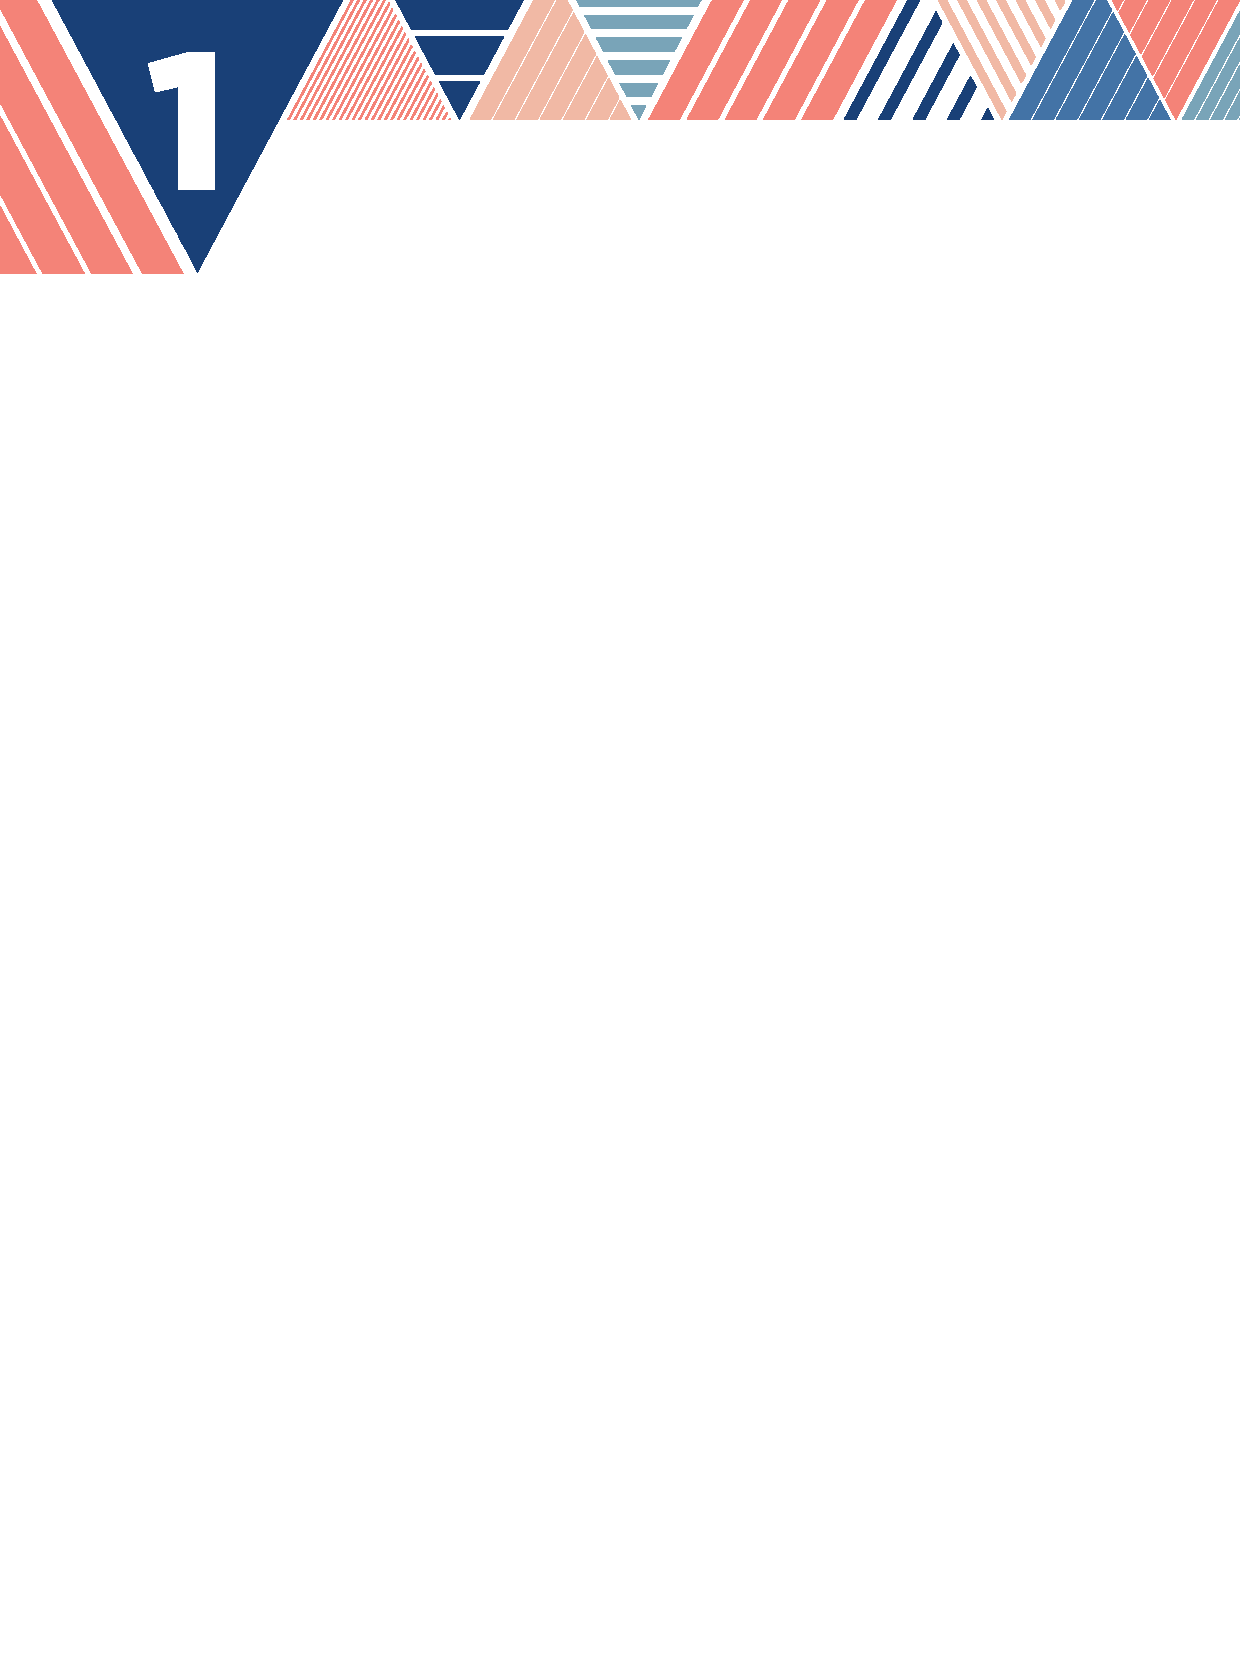
\includegraphics[scale=1]{../watermarks/1modulo9ano.pdf}}

\chapter{1. Práticas corporais: dos jogos eletrônicos aos esportes radicais}

\vspace*{-2\baselineskip}

%Felipe: quando havia problemas gramaticais nos textos utilizados (o que não foi incomum), fiz a correção e coloquei a expressão ``com alterações'' depois da citação. Em um dos textos, o autor suprimiu uma alusão a Dilma Roussef, mas essa supressão comprometia a compreensão do texto. Mantive a supressão, mas fiz pequena adaptação.    

\coment{Habilidades da BNCC: EF67EF01, EF67EF06, EF89EF03, EF89EF15, 
EF89EF18}

\colorsec{Habilidades do SAEB}

\begin{itemize}
\item
  Identificar as diferentes valências físicas necessárias
  à realização de práticas corporais (jogos eletrônicos, lutas, práticas
  corporais de aventura, ginásticas, esportes e dança).
\item
  Identificar o valor do patrimônio urbano e natural nas vivências das
  práticas corporais de aventura urbana e na natureza.
\item
  Identificar as características (códigos, rituais, elementos
  técnico-táticos, indumentária, materiais, instalações, instituições)
  das lutas.
\item
  Analisar as práticas corporais frente à disponibilidade de locais para
  sua vivência.
\item
  Analisar as transformações históricas, o processo de esportivização e
  a midiatização das práticas corporais, com ênfase nas lutas.
\end{itemize}

\reversemarginpar\marginnote{O objetivo deste módulo é habilitar o
estudante a entender o processo de esportivização e identificar as práticas
corporais presentes na sociedade, reconhecendo suas principais
características, e as valências físicas presentes nas
modalidades esportivas.\\}

\conteudo{As práticas corporais (jogos eletrônicos, ginásticas esportes, lutas,
danças etc.) são manifestações corporais presentes na sociedade. Em cada uma dessas atividades são trabalhadas as \textbf{valências físicas}, que são: \textbf{força} (vencer uma
carga externa), \textbf{velocidade} (realizar um movimento no menor
tempo possível), \textbf{resistência} (realizar o mesmo movimento por
vários segundos) e \textbf{flexibilidade} (capacidade de esticar uma
musculatura ao máximo).

Além disso, muitas práticas passam por um processo de \textbf{esportivização}, ou
seja, deixam de ser uma atividade voltada para o lazer e passam a ser um
esporte oficial. Suas características são:

\begin{itemize}
\item
  Presença de regras oficiais padronizadas;
\item
  Criação de órgãos oficiais para fiscalizar o esporte (federação e
  confederação);
\item
  Competições oficiais e treinamentos específicos.
\end{itemize}
}

\colorsec{Atividades}

\num{1} Escreva as capacidades físicas mais utilizadas em cada prática corporal:

\begin{escolha}
\item
  Corrida dos 100 metros: \coment{velocidade.}
\item
  Maratona: \coment{resistência.}
\item
  Ginástica artística: \coment{flexibilidade.}
\item
  Levantamento olímpico: \coment{força.}
\end{escolha}

\coment{Por meio desta atividade, o estudante vai
poder relacionar e identificar as capacidades físicas utilizadas em
algumas práticas corporais.}

\num{2} Relacione o tipo de práticas corporais de aventura (urbana ou
  natureza) com as modalidades apresentadas a seguir.

\begin{multicols}{2}

(\coment{1}) Slackline

(\coment{2}) Moutain bike

(\coment{2}) Corrida de orientação

(\coment{1}) Skate

\columnbreak

(1) Prática de aventura urbana

(2) Prática de aventura na natureza

\end{multicols}

\coment{O objetivo desta atividade é habilitar o estudante a
distinguir as práticas corporais realizadas nos ambientes urbanos das que 
ocorrem na natureza, valorizando os espaços para essas modalidades.}

\num{3} Observe a imagem a seguir:

\begin{figure}[htpb!]
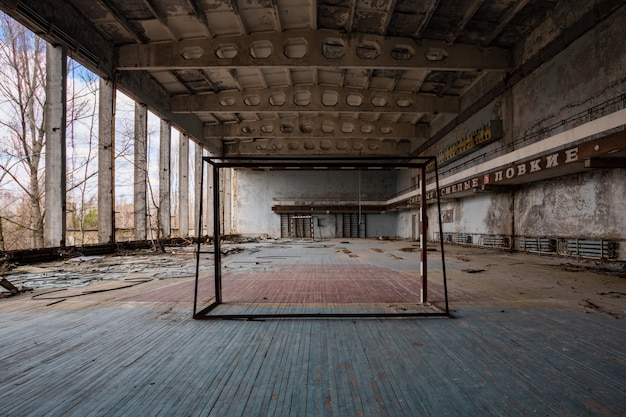
\includegraphics[width=2.99444in,height=1.99477in]{./imgs/img1.jpg}
\caption{Fonte: https://br.freepik.com/fotos-gratis/ginasio-abandonado-em-pripyat\_13499703.htm\#query=parque\%20abandonado\&position=6\&from\_view=search\&track=ais}
\end{figure}

Observando a imagem, é possível realizar alguma prática corporal? Qual é
o nosso dever em relação a esses espaços.

\linhas{3}

\coment{Na imagem, observa-se um ginásio esportivo abandonado, de
infraestrutura comprometida, cujo abandono, além de oferecer riscos
à saúde dos esportistas, inviabiliza o uso pela comunidade. O papel
das pessoas é preservar espaços públicos como esse, que podem ser 
extremamente benéficos quando adequadamente utilizados.
O propósito desta atividade é estimular o espírito crítico 
dos estudantes no que concerne aos espaços públicos disponíveis
na cidade.}

\num{4} No passado, o judô era uma luta voltada para a defesa pessoal.
  Atualmente é uma modalidade olímpica dividida em categorias, com 
  distinção de golpes proibidos e legítimos. É possível afirmar que essa
  luta passou por um processo de esportivização? Justifique sua
  resposta.

  %É adequado chamar o judô de "luta"? Minha experiência em escolas me ensinou que a expressão "arte marcial" é mais adequada (mas pode ser ignorância minha). (Rogério, 6/4/23, 13h08)

\linhas{3}

\coment{É correto afirmar que o judô passou pelo processo de
esportivização, pois, embora tenha sido um luta voltada para a autodefesa,
hoje em dia é um esporte com categorias, regras e golpes padronizados,
que são realizados em competições oficiais, como as Olimpíadas.

O objetivo dessa atividade é que o estudante
compreenda o processo por meio do qual uma prática corporal se torna 
um esporte oficial.}

\colorsec{Treino}

\num{1} Observe a imagem a seguir:

\begin{figure}[htpb!]
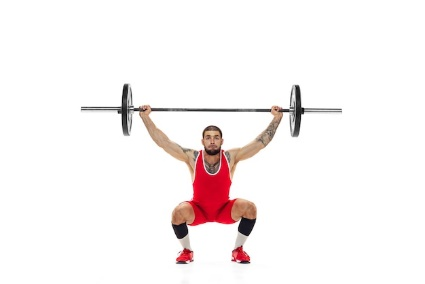
\includegraphics[width=1.92222in,height=1.28367in]{./imgs/img2.jpg}
\caption{Disponível em:
https://br.freepik.com/fotos-gratis/jovem-esportivo-treinando-com-barra-de-peso-isolada-sobre-fundo-de-estudio-branco-situps\_24908397.htm\#query=levantamento\%20de\%20peso\&position=41\&from\_view=search\&track=ais}
\end{figure}

Com base na imagem, o atleta está praticando uma modalidade que trabalha
a valência física de

\begin{escolha}
\item força, pois está vencendo uma carga externa que são as anilhas.

\item resistência, pois ficar agachado exige contração muscular das pernas.

\item velocidade, pois deve-se pegar a barra no chão e levantá-la para
cima.

\item flexibilidade, pois os músculos dos braços estão esticados.
\end{escolha}

\coment{SAEB: Identificar as diferentes valências físicas necessárias à
realização de práticas corporais (jogos eletrônicos, lutas, práticas
corporais de aventura, ginásticas, esportes e dança).

BNCC: EF67EF06 - Analisar as transformações na organização e na prática
dos esportes em suas diferentes manifestações (profissional e
comunitário/lazer).

a) Correta. de fato, a valência física trabalhada pelo atleta da imagem 
é a força, porque ele está vencendo uma caga externa composta por anilhas
e barra.
b) Incorreta. O levantamento olímpico trabalha a força, não a
resistência.
c) Incorreta. A velocidade não é praticada nesse esporte.
d) Incorreta. Nesse esporte, a flexibilidade não é priorizada.}

\num{2} Leia o texto a seguir:

\begin{quote}
O município de Salvaterra, no arquipélago paraense do Marajó, será palco
da estreia da luta marajoara nos Jogos Estudantis Paraenses (Jeps).

{[}...{]}

A típica luta marajoara é um combate corpo a corpo, que tem o objetivo
de projetar o oponente de costas ao chão e dominá-lo, esporte semelhante
ao Wrestling, praticado no norte do Brasil. Esta é a primeira vez que a
modalidade é incluída no torneiro, que está na sua 62ª edição.

\fonte{GE Pará. Salvaterra recebe os primeiros combates da luta marajoara
como modalidade do Jeps. Disponível em:
https://ge.globo.com/pa/noticia/salvaterra-recebe-os-primeiros-combates-da-luta-marajoara-como-modalidade-do-jeps.ghtml
. Acesso em: 6 abr. 2023.}
\end{quote}

Com base no texto, pode-se afirmar que a luta marajoara passou
por um processo de esportivização porque

\begin{escolha}
\item foram criados órgão oficiais relacionados a essa prática.

\item a prática está presente em um evento oficial.

\item o objetivo da prática foi alterado para a competição.

\item essa prática se assemelha à de um outro esporte.
\end{escolha}

\coment{SAEB: Analisar as transformações históricas, o processo de
esportivização e a midiatização das práticas corporais, com ênfase nas
lutas.

BNCC: EF89EF18 - Discutir as transformações históricas, o processo de
esportivização e a midiatização de uma ou mais lutas, valorizando e
respeitando as culturas de origem.

a) Incorreta. Não há alusão, no texto, à criação de
federações ou confederações da luta marajoara. 
b) Correta. A luta marajoara faz parte de um evento oficial de
competição, os Jogos Estudantis Paraenses.
c) Incorreta. Não há alusão, no texto, à alteração do objetivo da luta
marajoara. 
d) Incorreta. A semelhança entre a luta marajoara e o
wrestling não define essa prática corporal como esporte.}

\num{3} Leia o texto a seguir:

\begin{quote}
Skatistas de Curitiba terão, em breve, um novo espaço para praticar o
esporte. A Prefeitura de Curitiba começará a construir nos próximos 15
dias a maior pista pública de skate da cidade 

A pista, de 450 metros quadrados, será a primeira da região e é uma antiga 
reivindicação da população. O projeto feito pela Secretaria Municipal do 
Meio Ambiente teve a participação de skatistas. "Tomamos os cuidado de 
ouvir os praticantes do esporte e deixar o projeto o mais próximo possível 
da necessidade dos usuários", conta o superintende de obras e serviços da 
secretaria, Paulo Dalmaz.

%Felipe: consultei o original e alterei o trecho do texto escolhido. Na questão originla, a alternativa correta estava baseada em uma inferência duvidosa; entendo que, agora, a questão ficou mais consistente, além de enfatizar a demanda da população pelo esporte. (Rogério, 6/4/23, 13h45)

\fonte{Prefeitura Municipal de Curitiba. Nova pista pública de skate
será a maior da cidade. Disponível em:
https://www.curitiba.pr.gov.br/noticias/nova-pista-publica-de-skate-sera-a-maior-da-cidade/7410. Acesso em: 6 abr. 2023.}
\end{quote}

Após a leitura do texto, pode-se afirmar que o objetivo da construção da 
pista pública de skate é

\begin{escolha}
\item formar novos atletas para competições oficiais.

\item incentivar o uso de um novo meio de transporte.

\item atender à demanda da população pela prática do skate.

\item criar novos investimentos financeiros para a prefeitura.
\end{escolha}

\coment{SAEB: Identificar o valor do patrimônio urbano e natural
nas vivências das práticas corporais de aventura urbana e na natureza.

BNCC: EF67EF06 - Analisar as transformações na organização e na prática
dos esportes em suas diferentes manifestações (profissional e
comunitário/lazer).

a) Incorreta. Não há alusão, no texto, ao propósito de formar novos
atletas.
b) Incorreta. Não há alusão, no texto, ao uso do skate como meio
de locomoção. 
c) Correta. O segundo parágrafo é explícito quanto à demanda da 
população por um espaço adequado para a prática do esporte.
d) Incorreta. Não há alusão, no texto, ao propósito de criação de novos investimentos da prefeitura.}

\chapter{2. Esporte e dança}

\coment{O objetivo deste módulo é que o aluno compreenda as definições dos
esportes e entenda as características das danças, especificamente das
danças urbanas.\\

Habilidades da BNCC: EF67EF12, EF67EF13.}

\colorsec{Habilidades do SAEB}

\begin{itemize}
\item
  Diferenciar os esportes com base nos critérios de sua lógica interna.
\item
  Diferenciar as danças urbanas, seus elementos constitutivos e seu
  valor cultural nas demais manifestações da dança.
\end{itemize}

\conteudo{As \textbf{danças urbanas} desenvolveram-se em centros
urbanos ou periferias como forma de expressão e crítica social, por meio
do uso do corpo. É o caso da cultura do hip hop, que abarca traços
de diversas culturas e traz muitos benefícios para o praticante.

Além disso, muitas dessas danças, como o \textbf{breaking}, estão passando
pelo processo de esportivização e vão fazer parte de eventos oficiais,
como as Olimpíadas.}

\colorsec{Atividades}

\num{1} Relacione os elementos do hip hop (primeira coluna) com suas respectivas características (segunda coluna).

\begin{multicols}{2}

(1) Rap

(2) Breaking

(3) Grafite

(4) DJ

\columnbreak

(\rosa{2}) Dança do hip hop em que o dançarino pode improvisar os movimentos.

(\rosa{3}) Desenhos artísticos feitos em muros ou em paredes com spray.

(\rosa{1}) Canção do hip hop que tem improvisações e rimas.

(\rosa{4}) Pessoa responsável pela mixagem do som.
\end{multicols}

\coment{ O objetivo dessa atividade é que o aluno
identifique os elementos da cultura do hip hop.}

\num{2} Observe a imagem a seguir:

\begin{figure}[htpb!]
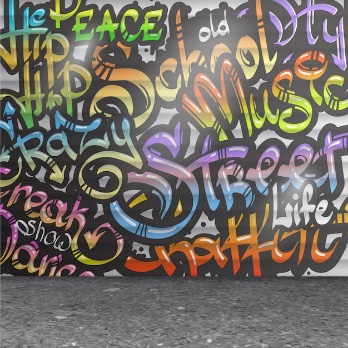
\includegraphics[width=1.57407in,height=1.57407in]{./imgs/img3.jpg}
\caption{Fonte: https://br.freepik.com/vetores-gratis/fundo-da-parede-de-graffiti\_4631697.htm\#page=2\&query=hip-hop\&position=47\&from\_view=search\&track=sph}
\end{figure}

Podemos dizer que a imagem mostra uma pichação? Justifique sua resposta.

\linhas{4}

\coment{Na imagem, observa-se não uma pichação, mas um grafite. 
O grafite é uma forma de arte visual cujos desenhos são feitos com spray,
normalmente realizados com autorização de prefeituras ou donos de
estabelecimentos. As pichações, por sua vez, são formas de vandalismo.}

%Felipe: acredito que a distinção entre grafite e pichação explicada no gabarito é, para dizer o mínimo, simplória. Além disso, deixa espaço aberto para nosso material ser alvo de duras críticas. Há quem defenda a pichação como forma de expressão. 

\num{3}  Marque com um X as danças que são consideradas como esportes oficiais.

\begin{boxlist}
\item Breaking. \coment{X}

\item Dança esportiva. \coment{X}

\item Maculelê.

\item Toré.
\end{boxlist}

\coment{O propósito desta atividade é facultar ao estudante a compreensão 
de que muitas danças podem ser consideradas como esporte oficial.}

\num{4}  Relacione as danças a seguir com suas respectivas origens.

\begin{multicols}{2}
(\coment{3}) Tango.

(\coment{1}) Hip hop.

(\coment{2}) Samba.

(\coment{4}) Dança esportiva

\columnbreak

(1) Dança urbana.

(2) Dança afro-brasileira.

(3) Dança de salão.

(4) Dança olímpica.
\end{multicols}

\coment{O objetivo dessa atividade é que o estudante identifique as
danças e sua origem.}

\num{5} Redija um texto curto explicando a origem da cultura hip hop
nas periferias das cidades dos Estados Unidos.

\linhas{4}

\coment{O hip hop surgiu nos guetos e bairros pobres dos Estados
Unidos como forma de protesto contra o racismo e a exclusão social.
Noos gêneros de canção, como o rap, de dança, como o break, e de artes 
visuais, como o grafite, eram formas de expressão da denúncia e das 
críticas dessa geração de artistas. 

O objetivo desta atividade é que aluno compreenda o contexto em que se 
originou a cultura hip hop.}

\colorsec{Treino}

\num{1} Leia a reportagem a seguir.

\begin{quote}
A revolução está aqui! Em Paris 2024, o breaking fará sua
estreia no programa dos Jogos Olímpicos. {[}...{]}

Serão três competições nas quais os atletas poderão garantir uma vaga
para a estreia do breaking em Paris 2024: o Mundial de 2023, os
jogos/campeonatos continentais e a série de classificatórios olímpicos.
{[}...{]}

Haverá dois eventos de breaking em Paris 2024 --- as competições
individuais masculina e feminina. Em cada um, 16 B-Boys e 16 B-Girls
lutarão para avançar para as próximas rodadas (ou pela medalha de ouro
na final) em batalhas solo cara a cara.

\fonte{Olympics. Rumo a Paris 2024: confira o sistema da classificação Olímpica do
breaking. Disponível em:
https://olympics.com/pt/noticias/sistema-de-classificacao-breaking-jogos-olimpicos-paris-2024.
Acesso em: 6 abr. 2023.}
\end{quote}

Considerando as informações do texto, pode-se afirmar que a dança citada
é esporte oficial porque

\begin{escolha}
\item prevê disputas por medalhas olímpicas.

\item fez parte das edições olímpicas anteriores.

\item inclui participação de homens e mulheres.

\item ter eventos de competições esportivas.
\end{escolha}

\coment{SAEB: Diferenciar os esportes com base nos critérios de sua lógica
interna.

BNCC: EF67EF12 - Planejar e utilizar estratégias para aprender elementos
constitutivos das danças urbanas.

a) Incorreta. A disputa por medalhas olímpicas não caracteriza se uma
modalidade é um esporte oficial ou não.
b) Incorreta. A dança urbana não foi modalidade esportiva de olimpíadas 
anteriores. A estreia ocorrerá em 2024.
c) Incorreta. A participação de homens e mulheres não caracteriza o
breaking como esporte oficial.
d) Correta. No texto, afirma-se que, além das Olimpíadas, os atletas
devem participar de outras competições oficiais.}

\num{2} Leia o texto a seguir.

\begin{quote}
A cultura hip hop é formada pelos seguintes elementos: o rap, o graffiti
e o break. {[}...{]}

Os três elementos juntos compõem a cultura hip hop, que muitos dizem que
é a ``CNN da periferia'', ou seja, que o hip hop seria a única forma da
periferia, dos guetos expressarem suas dificuldades, suas necessidades
de classes excluídas.

\fonte{Secretaria da Educação do Paraná. Dança de Rua. Disponível em:
http://www.educacaofisica.seed.pr.gov.br/modules/conteudo/conteudo.php?conteudo=60.
Acesso em: 6 abr. 2023.}
\end{quote}

Com base no texto, o hip hop surgiu como forma de

\begin{escolha}
\item expressão de adversidades.

\item incentivo à prática da dança.

\item criação de nova modalidade de dança.

\item assistência social do governo.
\end{escolha}

%Tive de alterar a primeira alternativa. O problema desta questão é o seguinte: o autor do material insiste no caráter de protesto do hip hop, mas o texto fala em expressão de dificuldades e necessidades. Protesto e expressão se aproximam, se tocam, mas não saõ necessariamente a mesma coisa. O problema é que o texto escolhido não diz o que o autor quer que ele diga. 

\coment{SAEB: Diferenciar as danças urbanas, seus elementos constitutivos
e seu valor cultural nas demais manifestações da dança.

BNCC: EF67EF13 - Diferenciar as danças urbanas das demais manifestações
da dança, valorizando e respeitando os sentidos e significados
atribuídos a eles por diferentes grupos sociais.

a) Correta. De acordo com o texto, no hip hop o rap, o grafite e
o break são formas de expressão das dificuldades dos moradores da 
periferia.
b) Incorreta. A origem do hip hop está mais associada à expressão das 
adversidades das pessoas da periferia do que ao incentivo à dança.
c) Incorreta. A origem do hip hop está mais associada à expressão das 
adversidades das pessoas da periferia do que à criação de uma nova
modalidade de dança.
d) Incorreta. Não há, no texto, referências ao hip hop como forma de 
assistência social do governo.}

\num{3}  Leia a reportagem a seguir.

\begin{quote}

Entre os ritmos apresentados, um que causou bastante animação na plateia
foi a performance de k-pop, gênero originário da Coreia do Sul, que
agrega elementos do pop, rock, hip hop, rap, reggae, street dance e
outras sonoridades contemporâneas.

\fonte{Notícias do Acre. Escola de Música do Acre e Balancé Balé promovem atividades de dança com
a comunidade. Disponível em:
https://agencia.ac.gov.br/escola-de-musica-do-acre-e-balance-bale-promovem-atividades-de-danca-com-a-comunidade/.
Acesso em: 21 fev. 2023.}
\end{quote}

Considerando a leitura do texto, é possível inferir que o k-pop pode ser
considerado como dança urbana por

\begin{escolha}
\item ter origem asiática.

\item ser realizado em grupos.

\item basear-se em movimentos corporais.

\item ter forte influência do hip hop.
\end{escolha}

\coment{SAEB: Diferenciar as danças urbanas, seus elementos constitutivos
e seu valor cultural nas demais manifestações da dança.

BNCC: EF67EF13 - Diferenciar as danças urbanas das demais manifestações
da dança, valorizando e respeitando os sentidos e significados
atribuídos a eles por diferentes grupos sociais.

a) Incorreta. A origem asiática do k-pop não implica que essa modalidade
seja considerada dança urbana.
b) Incorreta. A prática da dança em grupo não tem relação com sua
classificação com dança urbana.
c) Incorreta. Os movimentos corporais são constitutivos de quaisquer 
danças, de modo que essa característica não é suficiente para caracterizar 
o hip hop como danças urbanas.
d) Correta. O k-pop se inspirou em elementos do hip hop, como os
movimentos de dança do break e o rap.}

\chapter{3. Esporte na mídia}

\coment{O objetivo deste módulo é habilitar o estudante à análise 
crítica da presença do doping e da corrupção, em eventos esportivos, 
e à compreensão da mídia com padronizadora do corpo e consequentemente 
da saúde das pessoas.\\
Habilidades da BNCC: EF89EF08, EF89EF09.}

\colorsec{Habilidades do Saeb}

\begin{itemize}
\item
  Avaliar a multiplicidade de padrões de estética corporal disseminados
  pela mídia, que geram uma prática excessiva de exercícios e o uso de
  recursos ergogênicos.
\item
  Avaliar os problemas presentes nos esportes e abordados pela mídia,
  tais como doping, violência ou corrupção.
\item
  Avaliar a relação entre as práticas corporais e a promoção da saúde.
\end{itemize}

\conteudo{Os esportes são manifestações corporais presentes na sociedade.
Trata-se de práticas que trazem inúmeros benefícios a saúde física e 
mental das pessoas, como controle da massa corporal, socialização e
prevenção ao estresse. Porém, por causa de diversos motivos, como a ampla
cobertura da mídia e dos contratos milionários a ela relacionados, existem
pessoas que procuram obter resultados a qualquer custo, recorrendo a
práticas ilícitas como o doping e a corrupção.

Além disso, a mídia contribui para o discurso de padronização do corpo, 
ou seja, reproduz ideais de ``corpo perfeito e saudável'' que as 
pessoas, supostamente, deveriam ter. Essa busca incessante por um
modelo de perfeição, ao qual a maioria das pessas não corresponde,
é uma das causas de transtornos alimentares, como a bulimia.}

\colorsec{Atividades}

\num{1}  Relacione o nome dos transtornos alimentares com suas respectivas características.

\begin{multicols}{2}

(1) Anorexia.

(2) Bulimia.

(3) Vigorexia.

(4) Ortorexia.

\columnbreak

(\rosa{3}) Pessoa que se enxerga com baixa massa muscular.

(\rosa{4}) Pessoa que se preocupa exageradamente com a alimentação saudável.

(\rosa{1}) Pessoa que se enxerga com obesidade.

(\rosa{2}) Pessoa que induz o vômito.
\end{multicols}

\coment{O objetivo desta atividade é que o estudante reconheça e
identifique os principais transtornos alimentares que existem.}

\num{2} As competições, como as Copas do Mundo e as Olimpíadas, são
eventos esportivos que estão presentes na mídia, devido a altos
investimentos financeiros de governos e empresas privadas.
Consequentemente, há atletas que fazem de tudo para obter sucesso, 
incluindo práticas de corrupção e o uso de doping. Dessa maneira, 
escreva as definições desses dois problemas nos esportes.

\linhas{4}

\coment{No esporte, a \textbf{corrupção} corresponde à manipulação de
resultados por meio de recursos financeiros. O \textbf{doping} é o uso
de suplementos e anabolizantes ilegais para melhorar o condicionamento 
físico e, consequentemente, os resultados do atleta.

Por meio dessa atividade o estudante pode entender de maneira crítica 
alguns problemas presentes nos esportes no âmbito competitivo.}

\num{3} É de senso comum que qualquer prática esportiva traz benefícios 
para a saúde física e mental, como o fortalecimento muscular e a
socialização. Entretanto, é preciso conhecer o benefício específico de
cada esporte. Dessa maneira, relacione os esportes a seguir com seus 
principais benefícios.

\begin{multicols}{2}
(1) Pilates.\medskip

(2) Treinamento resistido.\medskip

(3) Natação.\medskip

(4) Corrida de 100 metros.

\columnbreak

(\coment{4}) Ajuda na capacidade física de velocidade.

(\coment{1}) Melhora a flexibilidade.

(\coment{2}) Aumento de massa magra.

(\coment{3}) Aumento da capacidade cardiovascular.
\end{multicols}

\coment{O propósito desta atividade é habilitar o estudante a
identificar e analisar os benefícios específicos de cada uma 
das práticas corporais.}

\num{4}  Observe a imagem a seguir:

\begin{figure}[htpb!]

\includegraphics[width=4.07407in,height=2.28999in]{./imgs/img4.jpg}
\caption{Fonte: https://br.freepik.com/psd-gratuitas/modelo-de-facebook-de-treinamento-de-musculacao-de-design-plano\_35720255.htm\#query=propaganda\%20academia\&position=16\&from\_view=search\&track=ais}
\end{figure}

É possível afirmar que a representação dos corpos nessa propaganda de 
academia corresponde à compleição física da maioria dos brasileiros?
Justifique sua resposta.

%Felipe: é o caso de pensarmos bem a respeito dessa questão. Tentei reformular o enunciado e o gabarito, mas gostaria de pensar junto a respeito. (Rogério, 12/4/23, 13h34)

\linhas{4}

\coment{Os corpos representados na propaganda não correspondem à 
compleição física da maioria da população brasileira. O que se observa
nessas imagens é uma padronização idealizada dos corpos, cujo modelo
é um modelo alto, magro, de músculatura extremamente definida e branco.

Por meio dessa atividade o estudante vai analisar e entender de maneira 
crítica a padronização idealizada dos corpos na propaganda.}

\colorsec{Treino}

\num{1} Leia o texto a seguir:

\begin{quote}
Comer é, sem dúvida, um dos prazeres da vida. Porém, quando a ingestão
de alimentos passa dos limites, o que deveria ser prazeroso torna-se um
pesadelo, que pode intervir diretamente na saúde física e mental do
indivíduo. {[}...{]}

{[}...{]} a pessoa também apresenta episódios de compulsão alimentar,
mas após estes momentos tem tanto medo de ganhar peso que acaba
adquirindo métodos para compensar e evitar o ganho de massa, como
vômitos, uso de laxantes, exercícios físicos em exagero e uso de
diuréticos''.

\fonte{Secretaria da Saúde do Estado do Ceará. Especialista orienta como identificar e tratar transtornos alimentares.
Disponível em:
https://www.saude.ce.gov.br/2019/09/05/especialista-orienta-como-identificar-e-tratar-transtornos-alimentares/.
Acesso em: 12 abr. 2023.}
\end{quote}

O transtorno alimentar descrito no segundo parágrafo do texto é a

\begin{escolha}
\item bulimia.

\item anorexia.

\item vigorexia.

\item ortorexia.
\end{escolha}

\coment{Saeb: Avaliar a multiplicidade de padrões de estética corporal
disseminados pela mídia, que geram uma prática excessiva de exercícios e
o uso de recursos ergogênicos.

BNCC: EF89EF09 -- Problematizar a prática excessiva de exercícios físicos
e o uso de medicamentos para a ampliação do rendimento ou
potencialização das transformações corporais, bem como os efeitos do
exercício físico para saúde e sua ausência, relacionada ao sedentarismo
e ao aparecimento de doenças.

a) Correta. A bulimia é caracterizada pela ingestão excessiva de alimentos
seguida pela indução de vômito pelo próprio indivíduo, para evitar
ganho de peso.
b) Incorreta. A anorexia se caracteriza por hábitos alimentares 
alterados, voltados sempre à perda de peso: privação de alimentos, 
dietas restritivas extremas, longos períodos em jejum, uso de 
medicamentos laxativos e inibidores de apetite, além de outros 
comportamentos, como excesso de práticas esportivas e vômitos
induzidos. 
c) Incorreta. A vigorexia é um transtorno no qual o indivíduo
tem de si mesmo uma imagem distorcida: embora tenha compleição
física forte e musculosa, diante do espelho ele se vê como fraco
e franzino.
d) Incorreta. A ortorexia é a obsessão pela alimentação saudável.}

\num{2} Leia a reportagem a seguir:

\begin{quote}
Uma das exigências para o Brasil sediar os Jogos Olímpicos e os Jogos
Paralímpicos de 2016 foi a criação de uma organização nacional
antidopagem. Assim, em 30 de novembro de 2011, foi criada a Autoridade
Brasileira de Controle de Dopagem (ABCD).

Integrada ao Ministério do Esporte, a ABCD é um dos grandes legados para
o país com a realização dos Jogos de 2016. A entidade é a responsável
pela implementação de uma política nacional de prevenção e de combate à
dopagem -- prática antiética de atletas que fazem uso de substâncias e
métodos proibidos, dentro e fora de competições, para potencializar o
desempenho.

\fonte{Rede do Esporte. Controle de dopagem. Disponível em:
http://rededoesporte.gov.br/pt-br/legado/antidopagem#. com alterações.
Acesso em: 12 abr. 2023.}
\end{quote}

Com base no texto, o \textit{doping} é definido como uma prática ilegal 
na qual os atletas

\begin{escolha}
\item treinam de maneira excessiva para uma determinada prova.

\item usam substâncias proibidas para ganhar as competições.

\item burlam as regras das competições oficiais.

\item evitam o uso de anabolizantes proibidos.
\end{escolha}

\coment{SAEB: Avaliar os problemas presentes nos esportes e abordados pela
mídia, tais como doping, violência ou corrupção.

BNCC: EF89EF09 -- Problematizar a prática excessiva de exercícios físicos
e o uso de medicamentos para a ampliação do rendimento ou
potencialização das transformações corporais, bem como os efeitos do
exercício físico para saúde e sua ausência, relacionada ao sedentarismo
e ao aparecimento de doenças.

a) Incorreta. O treino em excesso é definido como \textit{overtrainig},
e não como \textit{doping} ou dopagem.
b) Correta. A ingestão ou aplicação de substâncias proibidas caracteriza
o \textit{doping} ou dopagem, como se pode verificar no próprio texto.
c) Incorreta. A prática de burlar as regras não caracteriza o 
\textit{doping} ou dopagem, que está associado especificamente ao uso
de substâncias ilícitas. 
d) Incorreta. Quem evita o uso de anabolizantes proibidos não está
incorrendo na prática do \textit{doping} ou dopagem.}

\num{3}  Leia o texto a seguir:

\begin{quote}
{[}...{]} quem pratica esporte ou se exercita vive mais e melhor. ``A
prática esportiva traz longevidade e melhora a qualidade de vida. São
diversos os benefícios físicos e mentais: nosso ânimo melhora, temos
mais disposição, há liberação de hormônios importantes para o organismo,
e ajuda na parte estética, ou seja, troca a gordura por massa magra'',
explica Nathali Oliani, nutróloga e médica do esporte. O resultado é 
uma pessoa mais saudável e mais feliz.

\fonte{A importância do esporte para a qualidade de vida. Prefeitura Municipal
de Araraquara. Disponível em: https://wickbold.com.br/importancia-do-esporte-para-qualidade-de-vida/.
Acesso em: 12 abr. 2023.}
\end{quote}

%Felipe: aqui temos outro problema. A referência original do texto era o site da prefeitura de Araraquara, mas, pelo jeito, saiu do ar. Encontrei o mesmo texto no site da Wickbold, mas não sei se é adequado usar. Deixo a seguir a referência original https://www.araraquara.sp.gov.br/noticias/2017/10/a-importancia-do-esporte-para-a-qualidade-de-vida-1.     

Segundo o texto, as práticas esportivas  

\begin{escolha}
\item reduzem a longevidade.

\item aumentam taxas de gordura.

\item ampliam a qualidade de vida.

\item reduzem reações químicas no corpo.
\end{escolha}

\coment{SAEB: Avaliar a relação entre as práticas corporais e a promoção da
saúde.

BNCC: EF89EF08 -- Discutir, analisar e refletir criticamente as
transformações históricas dos padrões de desempenho, saúde e beleza,
considerando a forma como são apresentados nos diferentes meios
(científico, midiático etc.), identificando e reconhecendo a influência
da mídia nos padrões de comportamento do/no corpo.

a) Incorreta. Segundo o texto, as práticas esportivas aumentam a
longevidade.
b) Incorreta. Segundo o texto, as práticas esportivas contribuem para a 
redução das taxas de gordura, trocada por massa magra.
c) Correta. Segundo o texto, as práticas esportivas melhoram a 
qualidade de vida.  
d) Incorreta. Não há referências, no texto, à redução de reações químicas
no corpo.}

%No original, a questão me pareceu pouco amparada no texto, com inferências duvidosas. Minha versão é certamente mais fácil e pode ser melhorada, mas tem gabarito indiscutível, amparado no texto. Caso queiram, posso melhorar, trocando o texto. (Rogério, 12/4/23, 14h36) 

\chapter{Simulado 1}

\num{1} Observe a imagem a seguir

\begin{figure}[htpb!]
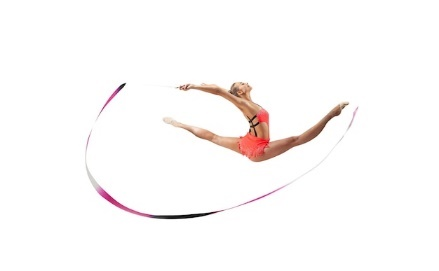
\includegraphics[width=1.98053in,height=1.22549in]{./imgs/img5.jpg}
\caption{Disponível em:
https://br.freepik.com/fotos-gratis/ginasta-ritmica-isolada-em-branco\_31843256.htm\#query=gin\%C3\%A1stica\%20art\%C3\%ADstica\&position=41\&from\_view=search\&track=ais.}
\end{figure}

A capacidade física utilizada no esporte apresentado é a

\begin{escolha}
\item força, pois a atleta está realizando um movimento com a sobrecarga da fita.

\item flexibilidade, pois a atleta está realizando uma abertura total das
pernas.

\item velocidade, pois a atleta deve movimentar rapidamente a fita.

\item resistência, pois a atleta está saltando tão alto quanto possível.
\end{escolha}

\coment{SAEB: Identificar as diferentes valências físicas necessárias à
realização de práticas corporais (jogos eletrônicos, lutas, práticas
corporais de aventura, ginásticas, esportes e dança).

BNCC: EF89EF03 -- formular e utilizar estratégias para solucionar os
desafios técnicos e táticos, tanto nos esportes de campo e taco,
rede/parede, invasão e combate como nas modalidades esportivas
escolhidas para praticar de forma específica.

a) Incorreta. Como é possível observar, a fita da ginástica é leve e não 
pode considerada como sobrecarga.
b) Correta. A flexibilidade consiste em alongamento máximo da musculatura, 
exatamente como se pode verificar na imagem. 
c) Incorreta. A imagem permite afirmar que, mesmo que movimente a fita com
rapidez, a ginasta exercita sobretudo a flexibilidade das pernas.
d) Incorreta. A resistência consiste na realização repetida do mesmo
movimento, não no salto mais elevado.}

\num{2} Leia o texto a seguir:

\begin{quote}
A tarde da última sexta foi um dia histórico para os skatistas
valadarenses, porque na ocasião a classe não só recebeu a notícia de
que a pista de skate da Feira da Paz será reformada como também pôde
falar sobre suas expectativas, discutir e sugerir propostas para o
projeto. {[}...{]}

O publicitário e skatista Diogo Lage foi à luta, procurou e indicou a
empresa especializada em pistas de skate para a Secretaria de Cultura, Esporte, Lazer e Turismo, levou o
arquiteto responsável pela elaboração dos projetos nas pistas e agora
está confiante. ``Com a reforma e revitalização do espaço, as famílias
poderão voltar a frequentar o local levando as crianças, e a comunidade
terá oportunidade de conhecer melhor o mais novo esporte olímpico. Com o
projeto concluído, os skatistas e o coletivo valadarense de skate farão a
Escolinha Social de Skate, que será uma oportunidade para tirar os
jovens do risco social da violência''.

\fonte{Prefeitura vai reformar a pista de skate. Prefeitura de Governador
Valadares. Disponível em:
https://www.valadares.mg.gov.br/detalhe-da-materia/info/prefeitura-vai-reformar-a-pista-de-skate/170101. com alterações.
Acesso em: 12 abr. 2023.}
\end{quote}

Com base no texto, os objetivos da reforma da pista de skate são

\begin{escolha}
\item lucrar com a prática de esportes urbanos e visibilizar a prática do skate.

\item formar atletas olímpicos no município e obter patrocínio privado para outros esportes.

\item atrair marcas que investem em skate e estimular a prática de esportes urbanos. 

\item atrair a comunidade para a prática do skate e usá-la como forma de prevenção à violência.
\end{escolha}

\coment{SAEB: Identificar o valor do patrimônio urbano e natural nas vivências
das práticas corporais de aventura urbana e na natureza.

BNCC: (EF67EF06): Analisar as transformações na organização e na prática
dos esportes em suas diferentes manifestações (profissional e
comunitário/lazer).

a) Incorreta. Não há referências, no texto, ao objetivo de lucrar com a prática de esportes urbanos.
b) Incorreta. O autor do texto se refere à apresentação do skate como novo esporte olímpico, sem se referir à formação atletas olímpicos ou ao patrocínio privado para outros esportes. 
c) Incorreta. Não há referências, no texto, à ``prática de esportes urbanos'', de forma genércia, nem ao objetivo de atrair marcas que investem em skate.
d) Correta. No trecho grafado entre aspas, no segundo parágrafo, verifica-se que a reforma da pista de skate servirá para aproximar a comunidade da prática desse esporte, além de contribuir para a prevenção da violência.}

\num{3}  Leia a reportagem a seguir:

\begin{quote}
Respeito e disciplina são a base de tudo. As outras regras que você
precisa saber para acompanhar o judô estão aqui.

\textbf{Tatame}\\
As lutas acontecem em um tatame quadrado, com medidas que variam de 14 a
16 metros.

\textbf{Uniforme}\\
Os judocas devem usar um quimono. Um dos atletas recebe uma faixa
vermelha, além da própria faixa, e é chamado de \textit{aka} (vermelho). O outro
recebe uma faixa branca e é chamado de \textit{shiro} (branco).

\textbf{Duração} da luta\\
As lutas têm duração de 4 minutos para o feminino sênior e sub-21, e de
5 minutos para o masculino sênior.

\fonte{Infraero. Regras. Disponível em:
http://www.infraero.gov.br/judo/regras/. Acesso em: 22 fev. 2023.}
\end{quote}

É possível afirmar que o judô passou pelo processo de esportivização,
porque, nessa arte marcial 

\begin{escolha}
\item não se distinguem categorias masculinas e femininas. 

\item o uso do quimono é condicionado à cor da faixa.

\item há padronização das regras e vestimentas.

\item valores éticos e morais são previstos no regulamento.
\end{escolha}

%Felipe: julgo que a versão original dessa questão era no mínimo discutível. A categorização do item a e a obrigatoriedade de uniforme do item b podem ser consideradas partes características do processo de esportivização, o que se confirma com o item c –– por isso mudei as alternativas.  

\coment{SAEB: Identificar as características (códigos, rituais, elementos
técnico-táticos, indumentária, materiais, instalações, instituições) das
lutas.

BNCC: (EF89EF18):~discutir as transformações históricas, o processo de
esportivização e a midiatização de uma ou mais lutas, valorizando e
respeitando as culturas de origem.

a) Incorreta. No judô existe distinção de categorias masculinas e femininas.
b) Incorreta. O uso do quimono é obrigatório, mas não é condicionado à cor da faixa. 
c) Correta. No processo de esportivização, há padronização de
regras e uniforme para as competições, como se pode verificar no texto.
d) Incorreta. Não há, no texto, quaisquer alusões à previsão de valores éticos e morais no regulamento.}

\chapter{Simulado 2}

\num{1} Leia o texto a seguir

\begin{quote}
O Ministério da Educação, por meio do Fundo Nacional de Desenvolvimento
da Educação (FNDE), tem liberado recursos para a construção de 6.116
quadras esportivas {[}...{]}

``Essa quadra foi um presente para a escola e para a comunidade'',
comemora a diretora Socorro Lima da Silva. Segundo ela, duas vezes por
semana alunos da Escola Municipal Walmik Sampaio de Albuquerque utilizam
a quadra da escola Vinícius de Morais para as aulas de educação física.
``Durante a semana, de 17h às 20h, a quadra é utilizada pela comunidade,
em jogos de futsal. E, nos fins de semana, é utilizada em atividades do
programa Escola Aberta, como eventos religiosos'', explica.

\fonte{ Ministério da
Educação. Escolas devem ser indicadas até setembro para ter quadras. Disponível em:
http://portal.mec.gov.br/ultimas-noticias/384-fnde-1801140772/18039-escolas-devem-ser-indicadas-ate-setembro-para-ter-quadras.
Acesso em: 12 abr. 2023.}
\end{quote}

Considerando as afirmações do texto, é possível inferir que a principal 
função da quadra da escola Vinícius de Morais é

\begin{escolha}
\item aumentar recursos financeiros da cidade.

\item incentivar a prática de esportes na comunidade.

\item promover competições oficiais de diferentes modalidades.

\item ampliar a frequência de eventos não esportivos.
\end{escolha}

\coment{SAEB: Analisar as práticas corporais frente à disponibilidade de locais
para sua vivência.

BNCC: (EF89EF03):~formular e utilizar estratégias para solucionar os
desafios técnicos e táticos, tanto nos esportes de campo e taco,
rede/parede, invasão e combate como nas modalidades esportivas
escolhidas para praticar de forma específica.

a) Incorreta. Não há alusão, no texto, à ampliação de recursos financeiros do município associados ao uso da quadra. 
b) Correta. A quadra da escola Vinícius de Morais é utilizada 
primordialmente para aulas de educação física e práticas esportivas.  
c) Incorreta. Não há alusão, no texto, à promoção de competições oficiais de diferentes modalidades.
d) Incorreta. Nos fins de semana, a quadra pode abrigar atividades não esportivas, mas essa não é sua principal função.}

\num{2} Leia o texto a seguir:

\begin{quote}
Para os povos da Antiguidade, o manuseio da espada era fundamental,
tendo em vista as constantes guerras e batalhas travadas.~ {[}...{]}

A Federação Internacional de Esgrima só foi criada em 1913. O primeiro
Campeonato Mundial da modalidade aconteceu em 1921, em Paris. Mas a
história da esgrima nos Jogos Olímpicos começou antes. Já em Atenas--1896
houve provas do esporte. Desde então, a esgrima nunca deixou de estar
presente em uma edição das Olimpíadas.

\fonte{Esgrima. Rede do Esporte. Disponível em:
http://rededoesporte.gov.br/pt-br/megaeventos/olimpiadas/modalidades/esgrima-1.
Acesso em: 12 abr. 2023.}
\end{quote}

Considerando as afirmações do texto, é possível afirmar que a esgrima é
um esporte oficial porque essa prática

\begin{escolha}
\item ocorre desde a Antiguidade.

\item é regulada por órgãos oficiais.

\item originou-se em guerras.

\item requer uso de instrumento específico.
\end{escolha}

\coment{SAEB: Analisar as transformações históricas, o processo de
esportivização e a midiatização das práticas corporais, com ênfase nas
lutas.

BNCC: (EF89EF18): Discutir as transformações históricas, o processo de
esportivização e a midiatização de uma ou mais lutas, valorizando e
respeitando as culturas de origem.

a) Incorreta. A prática centenária da esgrima não é condição suficiente 
para que essa prática seja considerada esporte oficial.
b) Correta. A regulação por federações ou confederações caracteriza a 
esgrima como esporte oficial. 
c) Incorreta. A origem bélica da esgrima não é condição suficiente 
para que essa prática seja considerada esporte oficial. 
d) Incorreta. O uso de instrumento específico, como a espada, não é
condição suficiente  para que essa prática seja considerada esporte 
oficial.}

\num{}  Leia a reportagem a seguir.

\begin{quote}
O Breaking Dance é um estilo que foi inserido recentemente entre as
modalidades das Olimpíadas e integrará os próximos jogos de Paris, na
França, em 2024. O tema vem movimentando as comunidades de danças
urbanas em todo o Brasil, esquentando o debate sobre a legitimidade do
Break como modalidade olímpica, tendo em vista ser considerado,
originalmente, um estilo de dança da cultura hip hop.

\fonte{Portal do Governo da Paraíba. Painel Funesc de dança traz debate
sobre o Break Dance nas Olimpíadas. Disponível em:
https://paraiba.pb.gov.br/noticias/painel-funesc-de-danca-traz-debate-sobre-o-break-dance-nas-olimpiadas.
Acesso em: 12 abr. 2023.}
\end{quote}

Com base no texto, é possível afirmar que o Breaking Dance

\begin{escolha}
\item deu origem à cultura hip hop.

\item tornou-se um esporte.

\item incentivou as competições de dança.

\item não pode ser chamado de dança urbana.
\end{escolha}

\coment{SAEB: Diferenciar os esportes com base nos critérios de sua lógica
interna.

BNCC: EF67EF13 -- Diferenciar as danças urbanas das demais manifestações
da dança, valorizando e respeitando os sentidos e significados
atribuídos a eles por diferentes grupos sociais.

a) Incorreta. A cultura hip hop deu origem ao Breaking Dance e outras
práticas corporais.
b) Correta. Pode-se afirmar que o Breaking Dance tornou-se esporte
porque será disputado em competição oficial. 
c) Incorreta. O autor do texto não menciona que o Breaking Dance tenha
incentivado competições de dança.
d) Incorreta. O Breaking Dance preserva as características de dança
urbana, mesmo que suas regras tenham sido padronizadas para as Olimpíadas.}

\chapter{Simulado 3}

\num{1}  Leia o texto a seguir:

\begin{quote}
Na condição de cultura urbana, o hip hop surgiu na periferia de Nova
York, entre as comunidades caribenhas, afro-americanas e
latino-americanas na década de 1970. O contexto social era de violência
e criminalidade nesses bairros, e a única forma de lazer possível para
os jovens era nas ruas. Encontraram na música, poesia, dança e na
pintura uma forma de manifestação de sua realidade e contestação.

\fonte{Governo do Estado do Ceará. Iniciação ao Hip hop desperta
interesse dos adolescentes no Projeto ``Danças Urbanas''. Disponível em:
https://www.seas.ce.gov.br/2021/08/05/iniciacao-ao-hip-hop-desperta-interesse-dos-adolescentes-no-projeto-dancas-urbanas/\#:\textasciitilde{}:text=Origem\%20do\%20Hip\%20Hop,os\%20jovens\%20era\%20nas\%20ruas.
Acesso em: 22 fev. 2023.}
\end{quote}

Considerando as informações da reportagem, é possível afirmar que o
hip hop surgiu com o objetivo de

\begin{escolha}
\item incentivar a prática esportiva em espaços abertos.

\item estimular o empreendedorismo social.

\item reduzir a violência na cidade por meio da arte.

\item contestar a realidade social de maneira pacifica.
\end{escolha}

\coment{SAEB: Diferenciar as danças urbanas, seus elementos constitutivos
e seu valor cultural nas demais manifestações da dança.

BNCC: EF67EF12 -- Planejar e utilizar estratégias para aprender
elementos constitutivos das danças urbanas.

a) Incorreta. O autor do texto não menciona o incentivo a práticas
esportivas como propósito da cultura hip hop. 
b) Incorreta. Não há referências, no texto, ao estímulo do empreendedorismo
social como propósito da cultura hip hop. 
c) Incorreta. A redução da violência por meio da arte não é mencionada, no 
texto, como propósito primordial do hip hop. 
d) Correta. Segundo o autor, o hip hop surgiu como forma de contestação 
das comunidades caribenhas, afro-americanas e latino-americanas na
década de 1970.}

\num{2}  Leia o texto a seguir.

\begin{quote}
Segundo o Blog da Saúde, a vigorexia é um tipo de transtorno dismorfóbico
-- de distorção da autoimagem {[}...{]}

Desse modo, a vigorexia é uma doença psicológica caracterizada pela
insatisfação constante com o corpo {[}...{]}

\fonte{Ministério da Saúde. Precisamos falar do excesso de atividade física: você sabe o que é
vigorexia? Disponível em:
https://www.gov.br/saude/pt-br/assuntos/saude-brasil/eu-quero-me-exercitar/noticias/2021/precisamos-falar-do-excesso-de-atividade-fisica-voce-sabe-o-que-e-vigorexia.
Acesso em: 12 abr. 2023.}
\end{quote}

A prática mais comum da pessoa acometida pela vigorexia é a

\begin{escolha}
\item obsessão pela alimentação saudável.

\item prática de exercícios físicos em excesso.

\item indução do vômito após uma refeição.

\item ingestão de pequenas quantidades de alimentos.
\end{escolha}

\coment{SAEB: Avaliar a multiplicidade de padrões de estética corporal
disseminados pela mídia, que geram uma prática excessiva de exercícios e
o uso de recursos ergogênicos

BNCC: EF89EF08 -- Discutir as transformações históricas dos padrões de
desempenho, saúde e beleza, considerando a forma como são apresentados
nos diferentes meios (científico, midiático, etc.).

a) Incorreta. A obsessão pela alimentação saudável caracteriza a ortorexia. 
b) Correta. A vigorexia é um transtorno no qual o indivíduo
tem de si mesmo uma imagem distorcida: embora tenha compleição
física forte e musculosa, diante do espelho ele se vê como fraco
e franzino. Por causa dessa distorção, ele insiste na prática de 
exercícios físicos em excesso, com a finalidade de obter a imagem 
de força.
c) Incorreta. A indução do vômito após uma refeição é comportamento típico de pessoas acometidas pela bulimia. 
d) Incorreta. A ingestão de pequenas quantidades de alimentos é comportamento típico de pessoas acometidas pela anorexia.}

\num{3}  Leia o texto a seguir

\begin{quote}
\textit{Doping} refere-se ao uso de substâncias naturais ou sintéticas
visando a melhora do desempenho dos atletas em competições. Este objetivo 
é ilícito e por isso são feitos testes de \textit{doping} durante competições.

\fonte{Secretaria da Educação. Doping. Disponível em:
http://www.ciencias.seed.pr.gov.br/modules/galeria/detalhe.php?foto=1845\&evento=1.
Acesso em: 22 fev. 2023.}
\end{quote}

Considerando a definição proposta no texto, pode-se inferir que os atletas
que praticam \textit{doping} são aqueles que

\begin{escolha}
\item evitam o uso de substâncias ilegais.

\item usam medicamentos proibidos para ganhar as competições.

\item pretendem recuperar-se de lesões.

\item aplicam os anabolizantes para cuidar da saúde.
\end{escolha}

\coment{SAEB: Avaliar os problemas presentes nos esportes e abordados pela
mídia, tais como doping, violência ou corrupção.

BNCC: EF89EF09 -- Problematizar a prática excessiva de exercícios
físicos e o uso de medicamentos para a ampliação do rendimento ou
potencialização das transformações corporais.

a) Incorreta. Atletas que evitam o uso de substâncias ilegais se afastam
da prática do \textit{doping}.
b) Correta. A alternativa corrobora a definição de \textit{doping} 
apresentada no texto. 
c) Incorreta. A prática do \textit{doping} não está associada a 
tratamentos médicos, mas à melhora do desempenho dos atletas em 
competições.
d) Incorreta. A prática do \textit{doping} não está associada
a cuidades de saúde,mas à melhora do desempenho dos atletas em 
competições.}

\chapter{Simulado 4}

\num{1} Leia o texto a seguir:

\begin{quote}
A atividade física é importante para o pleno desenvolvimento humano e
deve ser praticada em todas as fases da vida e em diversos momentos.
Além de apresentar inúmeros benefícios para a proteção e prevenção de
Doenças Crônicas Não Transmissíveis (DCNTs), a prática também tem
influência positiva nos aspectos psicológicos e sociais. Isso porque
muitas atividades coletivas incentivam a socialização, sendo esse um
elemento importante para todos, principalmente para crianças e
adolescentes, como parte da formação, assim como é um poderoso estímulo
para pessoas idosas.

\fonte{Ministério da Saúde. Conheça o primeiro Guia de Atividade Física para a População Brasileira. Disponível em:
https://www.gov.br/saude/pt-br/assuntos/saude-brasil/eu-quero-me-exercitar/noticias/2021/conheca-o-primeiro-guia-de-atividade-fisica-para-a-populacao-brasileira.
Acesso em: 22 fev. 2023.}
\end{quote}

Considerando as afirmações do texto, é possível afirmar que as atividades
físicas

\begin{escolha}
\item devem restringir-se a crianças, jovens e idosos.

\item agravam ocorrências de Doenças Crônicas Não Transmissíveis.

\item beneficiam não apenas as pessoas, mas também a sociedade.

\item impactam a saúde física, sem efeitos psicológicos.
\end{escolha}

\coment{SAEB: Avaliar a relação entre as práticas corporais e a promoção da
saúde.

BNCC: EF89EF08) -- Discutir as transformações históricas dos padrões de
desempenho, saúde e beleza, considerando a forma como são apresentados
nos diferentes meios (científico, midiático, etc.).

a) Incorreta. As atividades físicas devem ser preticadas em todas as
fases da vida. 
b) Correta. As atividades físicas previnem ocorrências de Doenças Crônicas Não Transmissíveis.
c) Correta. As atividades físicas trazem benefícios para as pessoas, 
em termos individuais, e para a sociedade como um todo.
d) Incorreta. As atividades físicas são benéficas para a saúde física e
psicológica.}

\num{2}  Leia a reportagem a seguir:

\begin{quote}
Iniciam amanhã, os Jogos Escolares Eletrônicos do Paraná. A 2ª edição da
competição acontecerá em 5 finais de semana nos meses de setembro e
outubro. A introdução do \textit{e-sports} nos Jogos Oficiais do Estado aconteceu
ano passado visando o intercâmbio e o entretenimento, aproximando os
alunos, como forma de atenuar os efeitos nocivos causados pela pandemia
da Covid-19.~{[}...{]}

Para a coordenadora dos Jogos Escolares do Paraná, Márcia Tomadon,
``tomamos esta medida para que todos os alunos possam participar. Muitas
vezes as escolas não conseguem montar uma equipe, então desta maneira
damos a possibilidade de todos estarem contemplados na competição, e
assim também já conseguimos uma interação entre crianças de escolas
diferentes''. Ela também ressaltou o bom número de alunos inscritos:
``foram 2.742 inscrições, um bom número tendo em vista que estamos
introduzindo o \textit{e-sports} na cultura esportiva escolar''.

\fonte{Paraná Esporte. Jogos Escolares Eletrônicos tem início neste sábado. 
Disponível em:
https://www.esporte.pr.gov.br/Noticia/Jogos-Escolares-Eletronicos-tem-inicio-neste-sabado.
Acesso em: 12 abr. 2023.}
\end{quote}

Considerando as informações apresnetadas na reportagem, é possível afirmar
que os \textit{e-sports}

\begin{escolha}
\item contribuíram para a integração dos alunos durante a pandemia.

\item estão passando pelo processo de se tornarem esporte oficial.  

\item causaram efeitos nocivos durante a pandemia.

\item reduziram a integração entre alunos de diferentes escolas.
\end{escolha}

\coment{SAEB: Identificar as diferentes valências físicas necessárias à
realização de práticas corporais (jogos eletrônicos, lutas, práticas
corporais de aventura, ginásticas, esportes e dança).

BNCC: EF67EF01) -- Experimentar e fruir, na escola e fora dela, jogos
eletrônicos diversos, valorizando e respeitando os sentidos e
significados atribuídos a eles por diferentes grupos sociais e etários.

a) Incorreta. A reportagem se refere a jogos interescolares que 
ocorreram depois da pandemia da Covid-19, como se pode inferir pela
leitura do primeiro parágrafo. 
b) Correta. O processo de tornar-se esporte oficial está associado a 
existência de competições oficiais, como os Jogos Escolares Eletrônicos.
c) Incorreta. A reportagem se refere a jogos interescolares que 
ocorreram depois da pandemia da Covid-19, como se pode inferir pela
leitura do primeiro parágrafo. 
d) Incorreta. Segundo as afirmações contidas no texto, os Jogos Escolares 
Eletrônicos contribuirão para a integração entre alunos de diferentes
escolas.}

\num{3}  Leia o texto a seguir:

\begin{quote}
Apesar de adorar dançar, Mara Raymundo começou a dançar como forma de
exercício físico para melhorar picos de pressão que tinha por conta da
vida agitada. ``Não queria tomar remédio, então fui dançar e hoje tenho a
pressão normal'', justifica Mara. Mas não foi só a pressão da Mara que
melhorou. ``A memória melhorou, decorando os passos da dança, e a relação
com os outros também, além do humor, do sono e da disposição. Me sinto
como se tivesse 15 anos'', comemora. Há um ano e meio ela dança duas
horas por dia, três vezes na semana, e ainda sai para dançar com os
amigos nos fins de semana. ``A música eleva, inspira'', completa.

\fonte{Ministério da Saúde. Dançar faz bem ao corpo, à alma e à mente. 
Disponível em:
https://www.gov.br/saude/pt-br/assuntos/saude-brasil/eu-quero-me-exercitar/noticias/2018/dancar-faz-bem-ao-corpo-a-alma-e-a-mente.
Acesso em: 12 abr. 2023.}
\end{quote}

Considerando as afirmações da reportagem, é possível afirmar que os 
benefícios da dança  

\begin{escolha}
\item estão condicionados ao uso de remédios prescritos.

\item levaram Mara ao desfrute da arte e à reclusão social.

\item impactaram a saúde física, mental e emocional de Mara.

\item revelaram que os problemas de pressão não eram reais.
\end{escolha}

\coment{SAEB: Avaliar a relação entre as práticas corporais e a promoção da
saúde.

BNCC: EF89EF15 -- Analisar as características (ritmos, gestos,
coreografias e músicas) das danças de salão, bem como suas
transformações históricas e os grupos de origem.

a) Incorreta. Não há alusão, no texto, ao condicionamento dos benefícios
da dança ao uso de remédios prescritos.
b) Incorreta. Mara não foi levada à reclusão social, ao contrário: sua 
vida social foi enriquecida pela dança.
c) Correta. Os benefícios da dança reduziram os picos de pressão, 
melhoraram a memória, o humor, o sono, a disposição e as relações de Mara 
com outras pessoas. 
d) Incorreta. A afirmação de que os problemas de pressão não eram reais 
não é corroborada pelo texto.}